\chapter{Analiz'a Teoretic'a}

\section{Introducere}

Pentru a asigura o bun'a desf'a'surare a activit'a'tii de dezvoltare 'si 'intre'tinere a oric'arui proiect, pentru a asigura flexibilitate la schimb'ari 'in domeniul cerin'telor 'si pentru a preveni hazarduri ulterioare, este necesar'a o analiz'a profund'a 'si am'anun'tit'a a proiectului 'si a componentelor sale 'inainte de 'inceperea implement'arii.

\medskip

Acest capitol descrie cerin'tele proiectului sub forma unor cazuri de utilizare, analizeaz'a arhitecturile bibliotecilor similare 'si prezint'a arhitectura propus'a prin descrierea componentelor ce urmeaz'a a fi implementate 'si rela'tiile dintre acestea.

\begin{itemize}
\item {\bf Cerin'tele proiectului} sunt structurate 'in cazuri de utilizare. 'Incep{\ia}nd cu analiza cerin'telor ne asigur'am ca proiectul atinge ni'ste scopuri bine definite f'ar'a a irosi timp 'in implementarea unor tr'as'aturi nenecesare. 'In plus, putem pleca de la cerin'tele ini'tiale pentru a scrie teste 'si a valida finalul proiectului.

\item {\bf Analiza arhitecturilor similare} presupune suprapunerea tehnologiilor deja existente peste cerin'tele proiectului 'si a decide dac'a deciziile luate 'in dezvoltarea altor arhitecturi se aplic'a la acest proiect. 'In cazul 'in care mai multe arhitecturi diferite se prezint'a favorabile, vom decide care este mai potrivit'a.

\item {\bf Descrierea componentelor} Proiectul final va fi compus din mai multe componente, fiecare av{\ia}nd rolul de a rezolva o anumit'a problem'a. Existen'ta 'si scopul acestor componente este dictat'a de cerin'tele proiectului 'si modul de implementare al acestuia. Prin descrierea compontelor urm'arim atingerea scopurilor bibliotecii enun'tate 'in cadrul cazurilor de utilizare.

\end{itemize}

\clearpage

\section{Cazuri de utilizare}

Pentru a modela cerin'tele proiectului, prezent'am urm'atoarele cazuri de utilizare ce au rolul de a documenta cerin'tele func'tionale ale bibliotecii wxStyle.

\begin{figure}[H]
	\centering 
	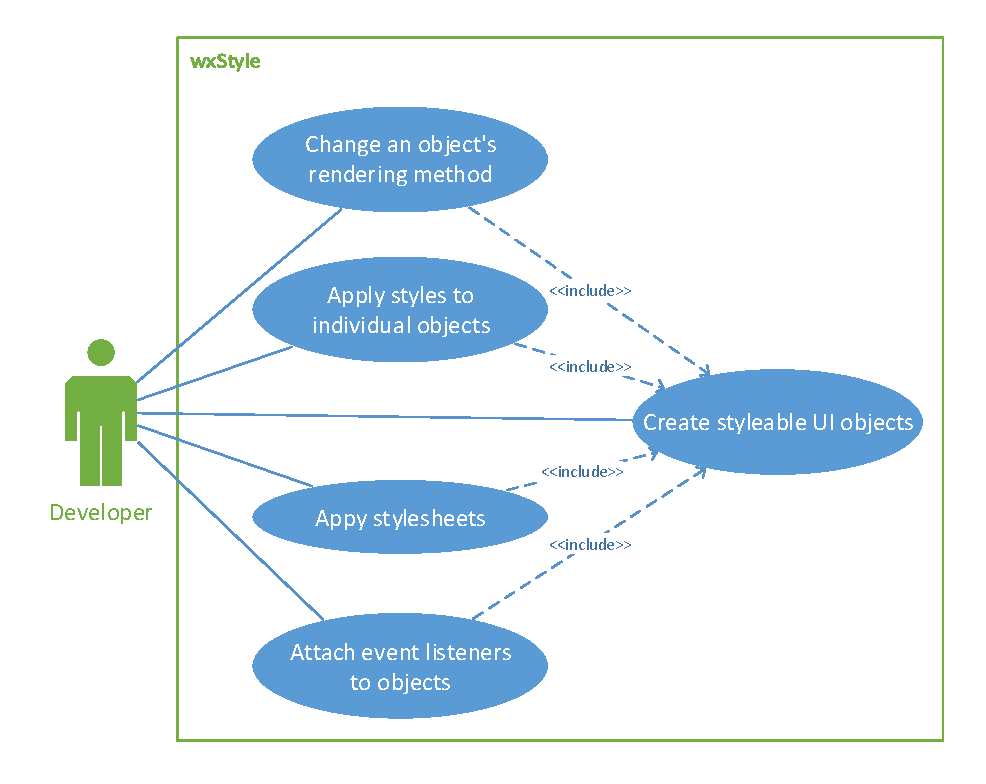
\includegraphics{img/use_case.pdf}
	\label{fig0401}
    \caption{Diagrama UML a cazurilor de utilizare}
\end{figure}

\subsection{Crearea unui obiect de interfa't'a}
\textbf{Precondi'tie:} Utilizatorul a configurat un mediu de dezvoltare care are acces la bibliotecile wxWidgets 'si wxStyle.
\begin{enumerate}
\item Utilizatorul preg'ate'ste o aplica'tie vizual'a wxWidgets prin implementarea 'si instan'tierea unui wxApp.
\item Utilizatorul declar'a o variabil'a cu unul din tipurile de date ale obiectelor stilizabile 'si 'ii asigneaz'a o instan'ta a acestui tip utiliz{\ia}nd constructorul.
\item Utilizatorul amplaseaz'a obiectul de interfa't'a 'in cadrul unei ferestre, utiliz{\ia}nd constr{\ia}ngeri de amplasare, printr-un proces identic cu amplasarea obiectelor de interfa't'a implementate in biblioteca wxWidgets.
\item Utilizatorul compileaz'a 'si ruleaz'a aplica'tia.
\end{enumerate}
\textbf{Rezultat:} Obiectul de interfa't'a este prezent in cadrul ferestrei.

\subsection{Stilizarea unui obiect de interfa't'a}
\textbf{Precondi'tie:} Parcurgerea cazului de utilizare intitulat \emph{Crearea unui obiect de interfa't'a}.

\begin{enumerate}
\item Utilizatorul construie'ste o instan't'a a clasei \emph{Style} 'si apeleaz'a metodele asociate cu setarea defini'tiilor de stilizare.
\item Utilizatorul ata'seaz'a stilul la un obiect de interfa't'a stilizabil.
\item Utilizatorul compileaz'a 'si ruleaz'a aplica'tia.
\end{enumerate}
\textbf{Rezultat:} Obiectul de interfa't'a este desenat conform defini'tiilor de stil specificate 'in structura de stil.

\subsection{Modificarea procesului de prezentare al unui obiect de interfa't'a}
\textbf{Precondi'tie:} Parcurgerea cazului de utilizare intitulat \emph{Crearea unui obiect de interfa't'a}.
\begin{enumerate}
\item Utilizatorul declar'a o nou'a clasa ce implementeaz'a interfa't'a numit'a \emph{Renderer}.
\item Utilizatorul implementeaz'a metoda \emph{Draw} a acestei clase folosind primitivele de desenare oferite de wxWidgets 'si instruc'tiunile de desenare oferite de wxStyle pentru a desena o reprezentare grafic'a a obiectului de interfa't'a conform st'arii acestuia.
\item Utilizatorul ata'seaz'a o instan't'a a acestei clase unui obiect de interfa't'a stilizabil.
\item Utilizatorul compileaz'a 'si ruleaz'a aplica'tia.
\end{enumerate}
\textbf{Rezultat:} Sistemul prezin'ta obiectul de interfa't'a 'in func'tie de starea sa 'si metoda de desenare implementat'a 'in cadrul clasei de prezentare.

\subsection{Schimbarea aspectului aplica'tiei}
\textbf{Precondi'tie:} Parcurgerea cazului de utilizare intitulat \emph{Crearea unui obiect de interfa't'a}.
\begin{enumerate}
\item Utilizatorul creaz'a op'tional mai multe obiecte de interfa't'a pe care le amplaseaz'a 'in cadrul unei ferestre.
\item Utilizatorul creaz'a o structur'a \emph{Stylesheet}.
\begin{enumerate}
  \item Utilizatorul construie'ste mai multe structuri de tipul \emph{Style} cu scopul de a le asocia unui tip de obiecte de interfa't'a.
  \item Utilizatorul ata'seaz'a stilurile structurii \emph{Stylesheet} 'si le asociaz'a c{\ia}te un nume unic.
  \item Utilizatorul face asocierea dintre tipul obiectului de interfa't'a 'si stilul dorit, ambele identificate prin numele lor, utiliz{\ia}nd metodele de asociere ale structuri \emph{Stylesheet}
\end{enumerate}
\item Utilizatorul aplic'a structura \emph{Stylesheet} prin inregistrarea sa la nivel global.
\end{enumerate}
\textbf{Rezultat:} 'In urma rul'arii aplica'tiei, toate obiectele de interfa't'a stilizabile ce nu au asociate stiluri sau clase de prezentare specificate de utilizator vor fi prezentate conform stilurilor asociate tipului lor din structura \emph{Stylesheet} 'inregistrat'a la nivel global.

\subsection{Procesarea evenimentelor}
\textbf{Precondi'tie:} Parcurgerea cazului de utilizare intitulat \emph{Crearea unui obiect de interfa't'a}.
\begin{enumerate}
\item Utilizatorul identific'a sursa evenimentului, care poate fi eveniment de interac'tiune utilizator sau eveniment generat de un obiect de interfa't'a.
\item Utilizatorul declar'a o nou'a clas'a care extinde interfa't'a de tip \emph{Listener} asociat'a evenimentului.
\item Utilizatorul implementeaz'a acea metod'a care proceseaz'a evenimentul dorit.
\item Utilizatorul ata'seaz'a o instan't'a a acestei clase unuia sau mai multora obiecte de interfa't'a.
\end{enumerate}
\textbf{Rezultat:} Metoda implementa't'a de utilizator este apelat'a 'in momentul producerii unui eveniment de tipul corect.

\section{Analiza arhitecturilor similare}

\subsection{Java Swing}

Biblioteca Swing a limbajului de programare Java pune la dispozi'tia utilizatorului o serie variat'a de obiecte de interfa't'a. Acestea utilizeaz'a predominant design pattern-ul MVC pentru decuplarea informa'tiei afi'sate de obiectul de interfa't'a ce prezint'a acea informa'tie.

\medskip

Aceasta bibliotec'a este de interes pentru proiect-ul de fa't'a datorit'a modurilor 'in care utilizatorul poate schimba 'inf'a'ti'sarea obiectelor de interfa't'a. Aceste moduri sunt:

\begin{enumerate}
\item Prin implementarea metodei \emph{paint(Graphics g)} se poate folosi obiectul \emph{g} pentru a invoca instruc'tiuni de desenare ce vor reprezenta obiectul de interfa't'a.
\item Prin 'inregistrarea unui obiect de tipul \emph{javax.swing.plaf.ComponentUI}\footnote{http://docs.oracle.com/javase/7/docs/api/javax/swing/plaf/ComponentUI.html} c'aruia i se va delega responsabilitatea de prezentare a tuturor obiectelor de interfa't'a de un anumit tip.
\item Unele obiecte de interfa't'a accept'a obiecte de tip \emph{Renderer} pentru a prezenta anumite p'ar'ti ale acestora. Un astfel de exemplu sunt celulele unui tabel ce pot fi desenate prin utilizarea unui \emph{TableCellRenderer}\footnote{http://docs.oracle.com/javase/7/docs/api/javax/swing/table/TableCellRenderer.html}.
\end{enumerate}

Prima metoda ne ofera libertate absolut'a 'in ceea ce prive'ste prezentarea obiectului de interfa't'a. Din p'acate, aceast'a metoda poate fi folosit'a doar pentru obiectele implementate de utilizator ce mo'stenesc ierarhia de clase Swing. Acest mod de stilizare este 'in general folosit pentru a construi obiecte inedite, pentru care este nevoia implement'arii unei clase individuale.

\medskip

Cea de-a doua metod'a permite dezvoltatorului stilizarea \emph{tuturor} obiectelor de interfa't'a de acela'si tip (de exemplu: a tuturor butoanelor). Aceast'a metod'a permite implementarea de teme complexe, numite \emph{Look and Feel}. Prin implementarea obiectelor de UI asociate fiec'arui tip de obiect de interfa't'a este posibil'a stilizarea 'intregii aplica'tii. Este important de re'tinut c'a aceast'a metod'a afecteaz'a obiectele native ale bibliotecii Swing, deci poate fi folosit'a cu u'surin'ta asupra programelor existente, f'ar'a a necesita utilizarea de obiecte de interfa't'a specializate.

\medskip

Ultima metod'a este util'a atunci c{ia}nd dorim s'a afect'am doar anumite p'ar'ti ale unui obiect de interfa't'a cum ar fi: celulele unui tabel, lista de elemente ale unui obiect de tipul \emph{combobox}, etc. 'In general, aceast'a metod'a este valabil'a obiectelor compuse, pentru a putea stiliz'a una sau mai multe sub-componente ale acestora.

\medskip

\subsection{Qt 'si Qt Stylesheets}

Biblioteca Qt este foarte similar'a cu biblioteca wxWidgets. Am{\ia}ndou'a au acela'si scop fundamenta: de a oferi o abstractizare uniform'a a obiectelor de interfa't'a pentru a construi cu u'surin't'a aplica'tii vizuale portabile 'in limbajul C++. Spre deosebire de wxWidgets, biblioteca Qt este 'intre'tinut'a de o corpora'tie, iar modurile 'in care aceasta poate fi folosit'a sunt determinate de doua tipuri de licen't'a: open source 'si cea comercial'a.

\medskip

Biblioteca Qt este de asemenea altfel implementat'a. Dac'a biblioteca wxWidgets manipuleaz'a obiecte de interfa't'a native sistemului de operare, biblioteca Qt implementeaz'a separat toate obiectele de interfa't'a independent de API-ul sistemului de operare. Diferen'ta vizibil'a dintre cele dou'a implement'ari este faptul c'a obiectele de interfa't'a a bibliotecii Qt pot fi prezentate 'in orice mod pe orice sistem de operare, deoarece opera'tia de prezentare este efectuat'a de biblioteca Qt, 'si nu de sistemul de operare.

\medskip

Similar bibliotecii Swing, Qt permite urm'atoarele moduri de schimbare a prezent'arii unui obiect:

\begin{enumerate}
\item Implementarea metodei \emph{paintEvent(QPaintEvent *event)}. Aceast'a metod'a este identic'a cu cea examinat'a in cadrul bibliotecii Swing, 'si nu o vom analiz'a mai departe.

\item Implementarea unui obiect de tipul \emph{QStyle}\footnote{http://qt-project.org/doc/qt-4.8/qstyle.html} ce are rolul de a prezenta orice obiect de interfa't'a.

\item Specificarea unui fi'sier de stil pentru a customiza o parte din caracteristicile vizuale ale obiectelor de interfa't'a.
\end{enumerate}

\medskip

Cea de-a doua metod'a presupune implementarea unui obiect ce are rolul de a prezenta orice obiect de interfa't'a. Modul 'in care acest obiect func'tioneaz'a este urm'atorul:

\begin{itemize}
\item Fiecare aspect al unui obiect este prezentat folosind una din metodele: \emph{drawItemText()}, \emph{drawItemPixmap()}, \emph{drawPrimitive()}, \emph{drawControl()}. Aceste metode pot fi utilizate 'si de c'atre obiectele de interfa't'a personalizate pentru a avea acela'si mod de prezentare ca restul obiectelor, pe orice platform'a. 
\item Metoda \emph{drawControl(ControlElement element, ...)} are rolul de a desena reprezentarea vizual'a a unui obiect de interfa't'a specificat prin identificatorul primit ca parametru. \emph{ControlElement} este un enum ce con'tine aproximativ 50 de valori, ce identific'a fiecare obiect de interfa't'a.
\item Metoda \emph{drawPrimitive(PrimitiveElement element)} are rolul de a desena un obiect "primitiv" precum indicatoarele de "+" 'si "-" ale unui spin box, sau s'age'tile unui tree view.
\item Numeroase enum-uri sunt disponibile pentru a identifica precis componenta sau subcomponenta ce trebuie desenat'a, pentru a specifica starea componentei 'si diverse op'tiuni de desenare.
\end{itemize}

De'si aceast'a metoda permite stilizarea 'intregii aplic'a'tii, similar cu modul 'in care biblioteca Swing accepta obiecte de tip \emph{UI}, implementarea unui astfel de obiect necesita tratarea tuturor obiectelor, 'si nu permite selectarea unei singure clase de obiecte care s'a fie uniform stilizate. 'In plus, proiectarea unei astfel de clase de stil necesit'a identificarea tuturor parametrilor necesari prezent'arii tuturor obiectelor, lucru foarte greu de realizat.

\medskip

Ultima metod'a 'imprumut'a no'tiunea de fi'siere de stil de la limbajul CSS pentru a oferi posibilitatea stiliz'arii dinamice la run-time a obiectelor de interfa't'a, utiliz{\ia}nd un limbaj specific acestui domeniu (DSL). Aceste specifica'tii de stil numite \emph{Qt Style Sheets}\footnote{http://qt-project.org/doc/qt-4.8/stylesheet.html} sunt compuse din secven'te de reguli. O regul'a de stil este la r{\ia}ndul ei compus'a dintr-un selector si o declara'tie. 

\subsubsection{Selectorul}

Selectorul are rolul de a selecta un set de obiecte de interfa't'a c'arora li se va aplica declara'tia de stil. Acest selector poate folosi tipul obiectelor de interfa't'a, numele acestora, dar si starea acestora. De exemplu, selectorul poate fi folosit pentru a selecta oricare din urm'atoarele mul'timi de obiecte: 
\begin{itemize}
\item Toate obiectele de interfa't'a ce acela'si tip. De exemplu: toate butoanele.
\item Un obiect specific de un anumit tip, identificat dupa numele acestuia. De exemplu: butonul "Add Client" care are asociat 'in cod numele "add\_client".
\item Se pot stiliza separat butoanele 'in starea ap'asat'a fa't'a de cele 'in starea normal'a.
\item Se pot stiliza individual componentele unui obiect de interfa't'a complex precum un combobox format dintr-un buton de selec'tie 'si o list'a de elemente, iar lista de elemente compus'a la randul ei din mai multe elemente.
\item Toate aceste criterii de selectare pot fi compuse pentru a forma criterii foarte specifice.
\end{itemize}

\subsubsection{Declara'tia de stil}

Declara'tia de stil este o list'a de propriet'a'ti ale obiectului de interfa't'a stilizat. Printre aceste propriet'a'ti putem enumera: culoarea fundalului, culoare primului plan, dimensiunea, font-ul, conturul, imaginea de fundal, icoana, etc. Aceste propriet'a'ti sunt specificate sub form'a de \emph{cheie: valoare} 'si sunt separate de caracterul \emph{;}. Este important de men'tinut c'a aceste stiluri se aplic'a la toate subclasele clasei selectate.

\medskip

Mecanismul de stilizare oferit de Qt este o adaptare a stilurilor CSS la obiectele de interfa't'a. Ele sunt limitate 'in ceea ce prive'ste num'arul 'si tipul de propriet'a'ti ce pot fi modificate, dar 'in acela'si timp 'indeplinesc foarte bine rolul de a separa modul de prezentare al unui obiect de implementarea acestuia. Mai mult, fi'sierele de stil pot fi specificate din linia de comand'a oric'arei aplica'tii Qt, indiferent de sursa acesteia.

\subsection{HTML 'si CSS}

Limbajul HTML este limbajul standard pentru prezentarea paginilor web. 'Impreun'a cu limbajul CSS ele pot fi utilizate pentru a specifica o gam'a larg'a de obiecte vizuale, 'impreun'a cu aranjarea acestora 'in pagin'a. Limbajul CSS este format dintr-o serie de specifica'tii de stil ce se pot aplica oric'aror obiecte HTML. Stilurile sunt compuse dintr-un selector si o declara'tie de stil. Selectorul este o expresie, posibil foarte complex'a, ce identific'a obiectele HTML c'arora li se va aplica stilul. Declara'tia de stil este o list'a de propriet'a'ti care vor fi setate obiectelor HTML.

\medskip

Aceste dou'a limbaje sunt relevante bibliotecii wxStyle, deoarece 'impreun'a formeaz'a prima tehnologie care permite stilizarea separat'a a obiectelor prin fi'siere de stil. Acest mecanism devine din ce 'in ce mai atractiv 'in tehnologiile moderne deoarece este foarte puternic dar 'si foarte u'sor de utilizat. 'In consecin't'a, exist'a un num'ar mare de dezvoltatori care cunosc HTML 'si CSS. O idee inovatoare de a utiliza acest mecanism 'in domeniul aplica'tiilor vizuale native a fost implementat'a de biblioteca Qt cu success moderat. Motivul pentru care fi'siere 'si declara'tiile de stil CSS nu au fost folosite mai devreme 'in aplica'tiile native este acela c'a stilurile CSS sunt menite a stiliza obiecte HTML statice, dreptunghiulare, lipsite de stare. 'In schimb, obiectele de interfa't'a au comportament 'si structur'a specific'a 'si sunt purt'atoare de stare. Obiectele de de interfa't'a pot fi stilizate doar par'tial, prin specificarea unor propriet'a'ti comune tuturor obiectelor.

\subsection{Formatul vectorial SVG}

Formatul vectorial SVG este un limbaj XML ce specific'a primitivele ce trebuiesc desenate. Astfel, se realizeaz'a o \emph{'int{\ia}rziere} a procesului de desenare p{\ia}n'a 'in momentul 'in care sunt cunoscute dimensiunile 'si suprafa'ta acestuia. Acest mod de reprezentare al imaginilor este atractiv pentru un mecanism de stilizare deoarece permite specificarea unui set de instructiuni de desenare ce vor fi interpretate de sistem 'in momentul prezent'arii unui obiect.

\medskip

Formatul SVG folose'ste descrieri ale unor obiecte pentru a le desena. Dintre tipurile acestor obiecte amintim:
\begin{itemize}
\item Geometrie format'a dintr-o serie de curbe si linii drepte.
\item Forme geometrice elementare: poligoane si elipse.
\item Paragrafe de text asupra c'arora se pot aplica efecte 'si care pot fi alinate la forme geometrice. De asemenea, se poate specifica fontul si dimensiunea textului.
\item Pensule de desenare al interiorului sau conturului acestor obiecte folosind culoare, imagini sau gradiente.
\end{itemize}

Aceste obiecte pot fi combinate pentru a genera imagini complexe. 'In domeniul bibliotecii wxStyle, aceste obiecte pot fi folosite ca instruc'tiuni de desenare specificate 'in fi'sierele de stil.

\subsection{Concluzie}

'In concluzie, tr'as'aturile pe care biblioteca wxStyle ar trebui s'a le aib'a sunt:
\begin{enumerate}
\item Stilizarea unei instan'te de obiect de interfa't'a. Acest lucru este posibil at{\ia}t in Swing c{\ia}t 'si in Qt prin implementarea unei clase nou'a de obiecte 'si suprascrierea metodei prezentare. Deoarece consider'am prea puternic'a aceast'a cerin't'a, dorim s'a oferim posibilitatea de a \emph{'inregistra} o procedura de prezentare unui obiect 'in mod dinamic. Acest lucru este posibil prin encapsularea procedurii de prezentare 'intr-un obiect. 'In acest mod putem reutiliza procedura de desenare 'si o putem aplic'a oric'arui obiect, indiferent de tipul acestuia.
\item Stilizarea unei clase de obiecte de 'interfa't'a. Acest lucru este posibil in Swing prin inregistrarea unui obiect de tip \emph{ComponentUI}, iar in Qt doar prin implementarea clasei \emph{Style}. Deoarece obiectele de interfa't'a ale bibliotecii wxStyle accept'a deja obiecte de prezentare, este posibil ca, 'in cazul 'in care un utilizatorul nu a 'inregistrat un prezentator unei instan'te, obiectele de interfa't'a s'a utilizeze un prezentator predefinit 'si accesibil global de c'atre toate instan'tele. Fiecare clas'a de obiecte de interfa't'a va avea un prezentator separat, care s'a poat'a fi interschimbat 'in timpul execu'tiei. Aceast'a alegere favorizeaz'a arhitectura bibliotecii Swing, deoarece este mai u'sor de utilizat de c'atre utilizatorii bibliotecii.
\item Stilizarea unei clase de obiecte sau a unei instan'te folosind stiluri. Am v'azut c'a este posibil'a definirea de stiluri prin perechi de tipul \emph{cheie: valoare} care s'a suprascrie propriet'a'ti ale obiectelor de interfa't'a. Aceste stiluri trebuiesc apoi utilizate 'in procesul de prezentare. 'In bibliotec'a wxStyle, urm'atoarele propriet'a'ti pot fi suprascrise prin stiluri: font, umbr'a, icoan'a, aliniament, fundal, culoare prim-plan, opacitate, margini. Pentru a putea beneficia de stiluri, fiecare obiect de interfa't'a va dispune de o instan'ta a unui stil. Aceast'a instan't'a poate sau nu sa fie utilizat'a de procedura de prezentare. Procedurile de prezentare predefinte de bibliotec'a vor utiliza instan'tele de stil.
\end{enumerate}

\section{Descrierea componentelor}

\subsection{Obiectele de interfa't'a}

Deoarece biblioteca wxWidgets nu suport'a suprascrierea prezent'arii unui obiect de interfa't'a, suntem nevoi'ti s'a implement'am obiectele stilizabile separat de obiectele de interfa't'a native wxWidgets. Obiectele de interfa't'a stau la baza bibliotecii wxStyle, deoarece f'ar'a ele nu putem stiliza nimic. Este totu'si important de observat c'a din acest motiv, aplica'tiile scrise deja folosind biblioteca wxWidgets nu vor putea beneficia de capabilit'a'tile bibliotecii wxStyle. Pentru ca aceste aplica'tii sa poat'a fi stilizate, putem opta s'a implement'am biblioteca wxWidgets deasupra obiectelor de interfa't'a stilizabile, a'sa cum ea este implementat'a deasupra obiectelor oferite de sistemul de operare.

\medskip

Obiectele de interfa't'a implementate de biblioteca wxStyle trebuie s'a suporte urm'atoarele tr'as'aturi:

\begin{itemize}
\item S'a accepte un prezentator 'si s'a-i delege responsabilitatea de desenare. 'In cazul 'in care un prezentator nu a fost setat explicit, s'a-l foloseasca pe cel implicit.
\item S'a accepte un stil. 'In cazul 'in care un stil nu a fost setat explicit, s'a-l foloseasc'a pe cel explicit.
\item S'a accepte observatori ai st'arii 'si evenimentelor sale. Pentru ca acest lucru s'a fie posibil, trebuie s'a construim un mecanism nou de procesare al evenimentelor, deasupra celui oferit de wxWidgets.
\end{itemize}

Pentru a putea fi utilizate 'in mod identic obiectelor de interfa't'a native wxWidgets, obiectele stilizabile vor trebui sa extinda ierarhia de obiecte de interfa't'a prin mo'stenirea celei mai generale clase.

\subsubsection{Procesare evenimentelor}
Motivul pentru implementarea unui alt mecanism de procesare al evenimentelor este de a oferi posibilitatea mai multor obiecte sa raspunda la evenimente. In momentul in care o rutina de procesare al evenimentului este legat'a de un anumit tip de eveniment si un anumit obiect, evenimentele de acel tip produse de acel obiect nu vor mai putea fi procesate de alta rutin'a. Acest lucru ingreuneaz'a biblioteca wxStyle, deoarece obiecte precum ResizeHandler 'si DragHandler trebuie sa poata intercepta evenimentele produse de dispozitiv-ul mouse f'ar'a a intrerupe propagarea acestora c'atre obiectul c'arora le este destinat. Dac'a aceste evenimente nu ar ajunge la obiectul destinatar, acesta nu ar putea s'a-'si actualizeze starea sau s'a genereze evenimente abstracte specifice obiectului precum ap'asarea unui buton sau mutarea indicatorului de text 'in interiorul unui obiect de interfa't'a pentru introducerea de text.

\begin{center}
\begin{figure}[h]
    \centering
    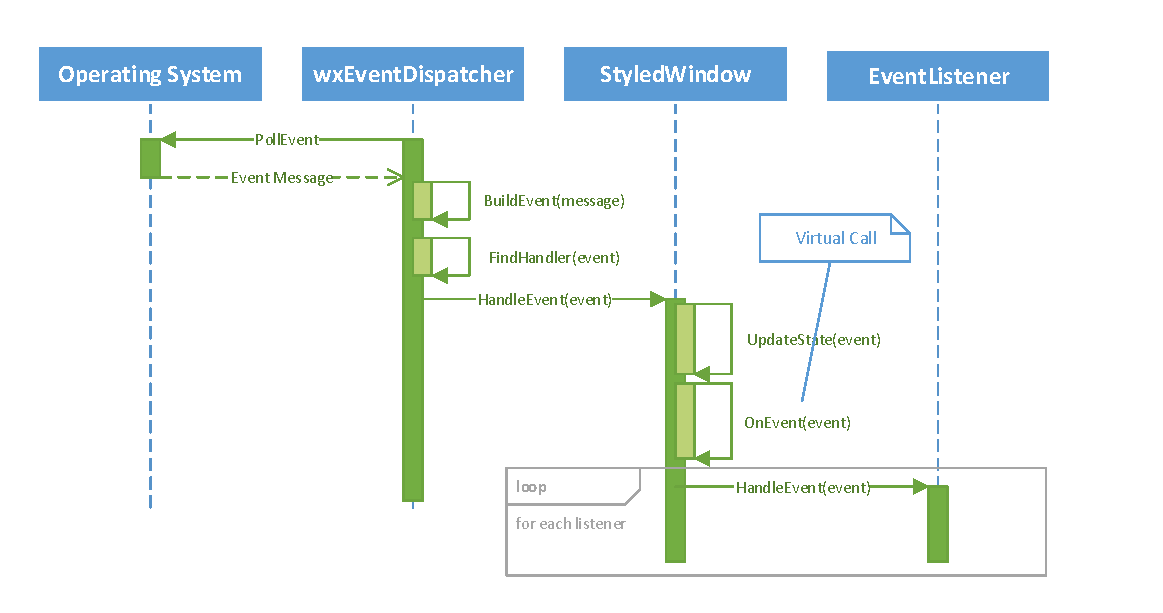
\includegraphics[scale=0.9]{img/seq_event_processing.pdf}
    \label{fig0402}
    \caption{Procesarea evenimentelor}
\end{figure}
\end{center}

Cel mai popular mecanism de distribuire a unui eveniment este cel bazat pe sablonul Observer. Acest mecanism presupune prezen'ta a dou'a componente: un produc'ator de evenimente 'si mai mul'ti 'ascult'atori de evenimente. Ascult'atorii se pot 'inregistra la produc'ator pentru a fi notifica'ti 'in cazul 'in care un nou eveniment este produs. La orice moment, un ascult'ator se poate deinregistra de la produc'ator. Produc'ator men'tine o list'a de ascult'atori. Ac'tiunile de inregistrare si deinregistrare se traduc 'in ac'tiuni de manipulare a listei precum ad'augarea unui noi observator sau 'stergerea unuia deja existent. Notificarea observatorilor presupune apelarea unei metode a obiectului observator. Aceste metode sunt predefinite de interfa't'a observatorului. Fiecare produc'ator accept'a doar un anumit tip de observator, pentru a asigura prezen'ta metodelor de procesare. 'In momentul gener'arii unui nou eveniment, produc'atorul notific'a toti observatorii. Utiliz{\ia}nd acest mecanism, putem procesa acela'si eveniment din locuri multiple.

\medskip

O problem'a la mecanismul de observator pentru procesarea evenimentelor este ordinea 'in care observatorii sunt notifica'ti de prezent'a unui eveniment. Dorim s'a ne asigur'am c'a obiectele de interfa't'a c'arora le este destinat evenimentul au ocazia s'a 'il proceseze 'inaintea altor observatori inregistrati de c'atre utilizatori. Din acest motiv, evenimentele sunt procesate 'in trei etape:

\begin{enumerate}
\item Clasa StyledWindow primeste evenimentul de la biblioteca wxStyle prin mecanismul standard wxWidgets. In cadrul acestei rutine, StyledWindow adjusteaz'a starea obiectului precum: dac'a este sau nu ap'asat, daca dispozitivul mouse se afl'a sau nu deasupra obiectului, etc.
\item StyledWindow apeleaza metoda virtuala On{Event} care este implementat'a (la nevoie) de tipul real al obiectului. In acest fel, obiectele de interfa't'a au ocazia s'a interpreteze evenimentele pentru a-'si 'intre'tine propria stare intern'a.
\item StyledWindow notific'a to'ti observatorii inregistra'ti pentru evenimentul respectiv. Ordinea 'in care ace'stia sunt notifica'ti este aceea 'in care ei s-au 'inregistrat.
\end{enumerate}

Deoarece clasa StyledWindow are responsabilitatea de a 'intre'tine starea obiectului, de a apela metoda virtual'a de procesare 'si de a notifica to'ti observatorii asigur'a corectitudinea proces'arii evenimentelor. Obiectele specifice de interfa't'a nu au responsabilitatea de a 'intre'tine o list'a de observatori sau de a procesa evenimentele 'intr-o anumit'a ordine.

\subsection{Prezentatorul}

Prezentatorul are rolul de a prezenta un obiect de interfa't'a. Prezentatorul este reprezentat de o interfa't'a cu o singur'a metod'a ce accept'a ca parametru obiectul de stilizat. Tipul parametrului este tipul generic al obiectelor de interfa't'a stilizabile. Din acest motiv, prezentatorul are access legal doar la metodele comune tuturor obiectelor de interfa't'a.

\begin{center}
\begin{figure}[h]
    \centering
    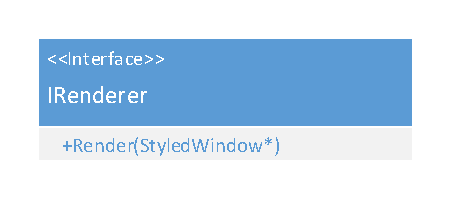
\includegraphics{img/irenderer.pdf}
    \label{ch2_arhitectura_bloc}
    \caption{Interfa'ta IRenderer}
\end{figure}
\end{center}

'In unele cazuri, c{\ia}nd se cunoa'ste exact tipul obiectului care va fi prezentat, parametrul trimis c'atre metoda \emph{Render} poate fi convertit ilegal printr-un downcast la tipul specific pentru a se putea accesa starea specifica acelui tip de obiect.

\subsection{Defini'tiile de stil}

Defini'tiile de stil 'in arhitectura \emph{Qt Style Sheets} 'si 'in limbajul CSS sunt 'imp'ar'tite 'in selector 'si declara'tie. Pentru simplitate, vom omite selectorul din arhitectura bibliotecii wxStyle. In schimb, vom oferi posibilitatea asocierii unui stil la o clas'a de obiecte de interfa't'a folosind o tabel'a separat'a. Astfel, defini'tiile de stil sunt individuale 'si reutilizabile. Stilurile vor fi reprezentate printr-o structur'a de date ce va re'tine toate specifica'tiile stilului. Aceast'a structur'a de date va putea fi \emph{combinat'a} cu o alt'a structur'a pentru a construi un stil din cele dou'a stiluri suprapuse. Stilurile vor putea fi 'inc'arcate dintr-un fi'sier de stil. Reprezentarea prin fi'sier de stil va folosi limbajul XML pentru simplitatea citirii 'si interpret'arii.

\begin{center}
\begin{figure}[h]
    \centering
    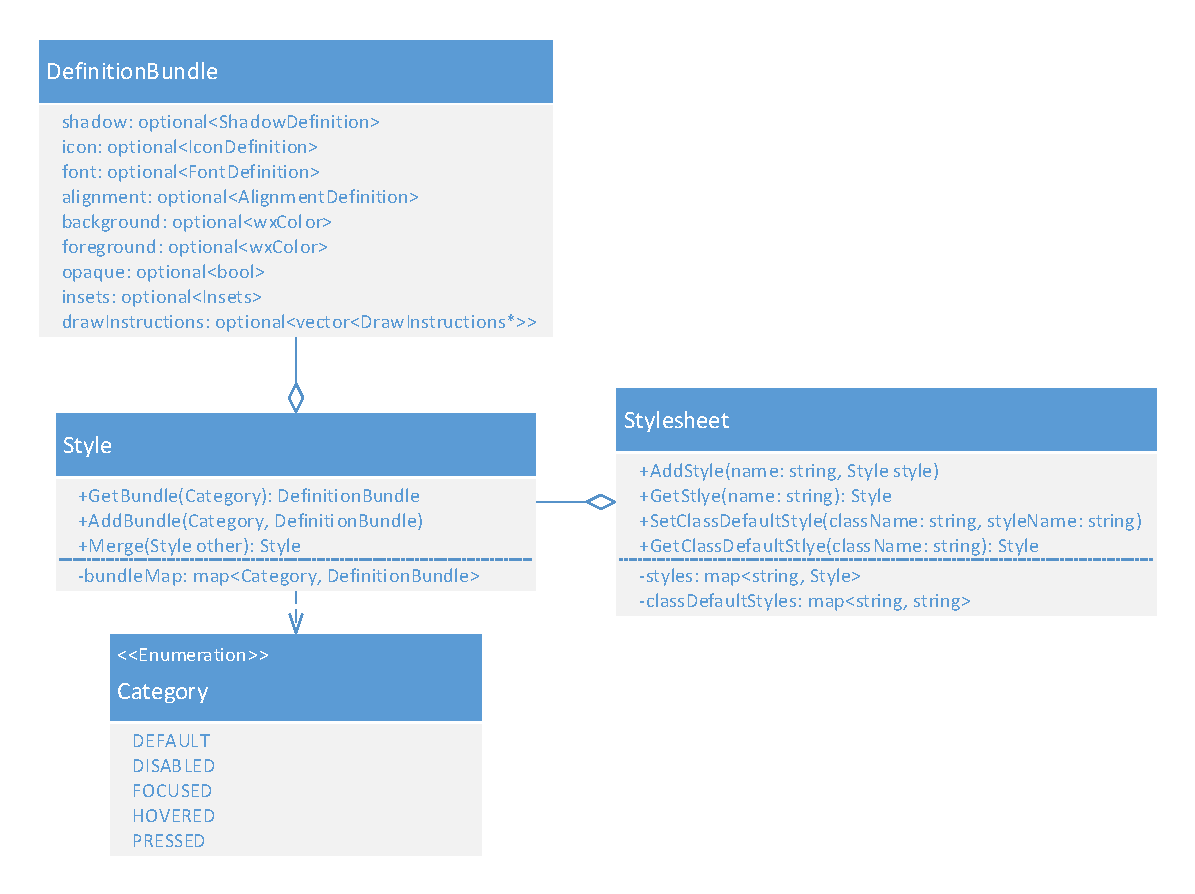
\includegraphics[scale=0.8]{img/uml_class_stylesheet.pdf}
    \label{fig0412}
    \caption{Diagrama de clase UML pentru defini'tiile de stil}
\end{figure}
\end{center}

O defini'tie de stil va fi compus'a din:
\begin{enumerate}
\item Numele stilului, unic in fi'sierul de stil 'in care este definit.
\item P'arintele stilului. Pentru a m'ari nivelul de reutilizare, 'si pentru a \emph{simula} mecanismul de cascadare al stilurilor prezent 'in \emph{Qt Style Sheets} 'si CSS, toate defini'tiile unui stil pot fi mo'stenite de la alt stil.
\item O list'a de defini'tii de propriet'a'ti 'imp'ar'tite pe categorii. 'In acest mod putem specifica stiluri diferite pentru st'arile obiectelor: \emph{default}, \emph{hovered}, \emph{pressed}, \emph{disabled}.
\end{enumerate}

Structura de date responsabil'a pentru reprezentarea unei defini'tii de stil va trebui s'a poat'a con'tine defini'tii par'tiale, astfel 'inc{\ia}t doar un subset de propriet'a'ti s'a fie descrise. 'In acest mod putem folosi mecanismul de combinare 'si cel de mo'stenire.

\subsubsection{Stilul implicit}
Pentru a putea utiliza u'sor 'si sigur mecanismul de stilizare, avem nevoie de garan'tia c'a defini'tiile obligatorii ale unui stil exist'a. Defini'tiile obligatorii sunt acele defini'tii f'ar'a de care nu se poate construi o reprezentare a obiectului de interfa't'a. De exemplu: defini'tiile pentru font, culoarea planului prioritar (foreground), combina'tia de defini'tii care descriu opacitatea 'si modul de prezentare al fundalului. Aceste defini'tii, dac'a nu sunt explicit setate, trebuie s'a aibe o valoare predefinit'a. Aceast'a valoare predefinit'a provine de la stilul implicit al bibliotecii wxStyle. Prin mecanismul de mo'stenire al stilurilor, toate defini'tiile setate manual de utilizator se vor aplica deasupra stilului implicit. 

\medskip

De asemenea, mecanismul de stilizare prin fi'siere de stil \emph{stylesheets} trebuie sa poata stiliza 'intreaga aplica'tie la orice moment 'in timpul rul'arii acesteia. Acest lucru presupune modificarea tuturor obiectelor de interfata ce nu au stiluri sau proceduri de prezentare predefinite din componen'ta aplica'tiei. Implementarea acestui mecanism poate fi facut'a 'in dou'a moduri:

\begin{enumerate}
\item Prin men'tinerea unei liste de obiecte vizuale care s'a con'tin'a toat'e obiectele de interfa't'a din componen'ta aplica'tiei. La momentul stiliz'arii aplica'tiei, toate obiectele din list'a vor fi parcurse, iar stilurile sau metodele lor de prezentare vor fi actualizate.
\item Prin men'tinerea unei liste de stiluri implicite, indexate dup'a tipul obiectului de interfa't'a c'aruia 'ii sunt asociate. Schimbarea stilului aplica'tiei implic'a updatarea stilulurilor din aceast'a lista. La momentul prezent'arii unui obiect ce nu are un stil sau un obiect de prezentare definit de utilizator, acesta interogheaz'a lista de stiluri 'si obiecte de prezentare standard.
\end{enumerate}

Metoda num'arul 1 implic'a stocarea 'in memorie a tuturor instan'telor de obiecte vizuale din aplica'tie, 'intr-o structur'a de date de tip list'a. Aceast'a list'a este greu de 'intre'tinut deoarece obiectele trebuiesc 'sterse din list'a 'in momentul 'in care acestea sunt distruse. Mai mult, modificarea unui stil predefinit implic'a parcurgerea 'intregii liste, indiferent dac'a obiectul este vizibil sau nu. Totu'si, lista va fi parcurs'a o singur'a dat'a pentru fiecare schimbare 'in setul de stiluri predefinite ale aplica'tiei. De cele mai multe ori, acest lucru se va realiza de doua ori: prima data pentru setarea stilului implicit al bibliotecii, iar a doua oara pentru setarea stilurilor specificate implicit de c'atre utilizator. Pentru a nu suprapune stilul implicit peste un stil setat de utilizator, toate obiecte de interfa't'a vor trebui augmentate cu un membru boolean care s'a indice dac'a stilul sau obiectul de prezentare al obiectului de interfa't'a este sau nu setat explicit de c'atre utilizator.

\medskip

Metoda num'arul 2 are avantajul c'a nu necesit'a men'tinerea unei structuri de date suplimentare pentru stocarea instan'telor obiectelor de interfa't'a. 'In schimb, aceast'a metoda presupune stocarea stilurilor, 'si delegarea opera'tiei de citire a stilurilor c'atre fiecare obiect de interfa't'a. In mod similar primei metode, aceast'a metod'a necesit'a augmentarea cu membrul suplimentar care s'a disting'a dintre stiluri si obiecte de prezentare setate de utilizator, si cele implicite. Doar obiectele ce nu au stiluri setate explicit vor apela la cele implicite. Accesul la stilurile si obiectele de interfa't'a implicite se poate face printr-o instan'ta global'a 'si unic'a a unei clase ce are singurul rol de a stoca aceast'a informa'tie. O alt'a metod'a este de a oferi tuturor obiectelor de interfa't'a o instan'ta a unei clase ce poate "produce" stiluri si obiecte de prezentare specializate pentru tipul obiectului de interfa't'a. Folosim verbul "produce", deoarece dorim ca instantele de stiluri sa poat'a varia 'in timpul rul'arii, deci nu putem trimite instan'te concrete. Mai degrab'a trimitem un obiect care poate construi instan'te variabile 'in timpul rul'arii.

\subsection{Prezentatorul de stiluri 'si instructiunile de desenare}

\subsubsection{Prezentatorul de stilur}

Acest prezentator este un prezentator specializat care utilizeaz'a informa'tia de stil a unui obiect de interfa't'a pentru a genera reprezentarea vizual'a a acestuia. Deoarece obiectele de interfa't'a diferite reprezint'a modele de date diferite 'si interac'tioneaz'a cu utilizatorul 'in moduri diferite, ele vor necesita implement'ari diferite ale prezentatorului.

\medskip

Fiecare tip de obiect de interfa't'a va avea setat implicit un prezentator implementat de libr'arie care s'a fie sensibil la specifica'tiile stilului. 'In acest mod, toate obiectele de interfa't'a vor reac'tiona corect 'si 'in mod implicit la modific'arile de stil. Una din atribu'tiile comune tuturor prezentatorilor de acest fel, indiferent de tipul obiectului de interfa't'a pe care 'il prezint'a este desenarea fundalului. Deoarece toate stilurile pot specifica proprietatea de opacitate 'si instruc'tiuni de desenare a fundalului, este normal ca aceast'a opera'tie s'a fie implementat'a 'intr-un singur loc. Locul potrivit pentru aceasta este clasa p'arinte pentru toti prezentatorii de stil.

\subsubsection{instructiunile de desenare}

Instruc'tiunile de desenare sunt un mecanism versatil care combin'a puterea metodei de stilizare prin implementarea unui prezentator 'si simplitatea de utilizarea a fi'sierelor de stil. Instruc'tiunile de utilizare profit'a de observa'tia c'a o implementare tipic'a a unei metode de desenare prin implementarea unui prezentator este o simpl'a secven't'a de instruc'tiuni de desenare a formelor geometrice primitive, a imaginilor sau a textului. Aceste instruc'tiuni pot fi codificate in limbajul XML cu u'surin't'a, fapt demonstrat de formatul vectorial SVG. 

\begin{figure}[h]
    \centering
    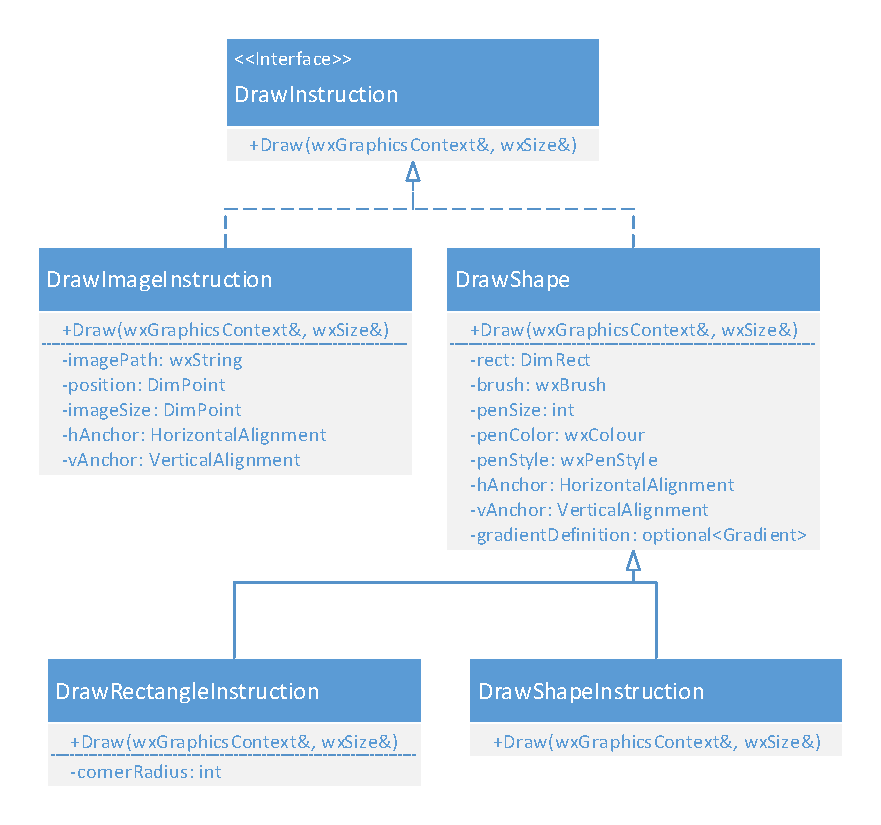
\includegraphics{img/uml_class_draw_instructions.pdf}
    \label{fig0403}
    \caption{Diagrama de clase a instruc'tiunilor de desenare}
\end{figure}

'In plus fat'a de instruc'tiuni de desenare, un prezentator scris 'in limbajul C++ mai are acces 'si la starea obiectului. El poate folosi instruc'tiuni condi'tionale pentru a schimba modul de prezentare al unui obiect de interfa't'a 'in func'tie de starea acestuia. Pentru a beneficia de aceste posibilit'a'ti 'in cadrul unui fi'sier de stil, avem nevoie de dou'a lucruri:

\begin{enumerate}
\item Un mod de a acesa starea obiectului stilizat.
\item Un mod de a condi'tiona setul de instruc'tiuni de desenare 'in func'tie de starea obiectului.
\end{enumerate}

Prima cerin't'a poate fi 'indeplinit'a prin introducerea unui mecanism de extragere a propriet'a'tilor cu nume a unui obiect. Aceste propriet'a'ti pot 'inlocui valori 'in cadrul instruc'tiunilor de desenare. Spre exemplu: pentru a desena textului unui label, vom utiliza o instruc'tiune de desenare \emph{DrawText} al c'arei parametru \emph{text} va fi egal cu proprietatea \emph{text} a obiectului de interfa't'a. Pentru a avea acces la propriet'a'tile obiectelor de interfa't'a, acestea trebuie s'a prezinte o map'a de tipul cheie: valoare, unde cheia este numele propriet'a'tii, iar valoarea este valoarea efectiv'a a acelei propriet'a'ti. Deoarece propriet'a'tile pot avea un numar diferit dar limitat de tipuri, este necesar'a utilizarea unui tip mai generic pentru reprezentarea valorilor.

Cea de-a doua cerin't'a poate fi indeplinit'a prin introducerea unui singur element XML, acela de condi'tie. Atributele acestui element pot specifica o expresie care folose'ste propriet'a'tile unui obiect.

\medskip

Pentru simplitate, vom alege s'a implement'am doar ce-a de-a doua cerin't'a, f'ar'a a putea 'ins'a specifica expresii bazate pe starea obiectului. In schimb, 'in cadrul unui stil, vom avea mai multe sub-elemente XML pentru fiecare din st'arile elementare ale unui obiect: \emph{default}, \emph{pressed}, \emph{hovered}, \emph{disabled}. Propriet'a'tile definite 'in cadrul categoriei \emph{default} vor fi combinate cu cele definite 'in celelalte st'ari pentru a genera un stil final al obiectului 'in orice stare. Aceast'a implementare este mult mai simpl'a dec{\ia}t cele analizate mai devreme, dar este 'si mult mai u'sor de implementat. 'In ciuda simplit'a'tii sale, aceast'a metod'a este suficient de versatil'a pentru majoritatea cazurilor.

\medskip

Pe viitor se poate extinde limbajul de stilizare cu ad'augarea posibilit'at'ii de interogare a st'arii obiectului de interfa't'a stilizat 'si selec'tia instruc'tiunilor de desenare.

\subsection{Ferestre}

Stilizarea ferestrelor este o tr'as'atura specific'a bibliotecii wxStyle, ea neexist{\ia}nd 'in nici-o alt'a bibliotec'a sau arhitectur'a analizat'a. Prin stilizarea unei ferestre ne dorim s'a puntem specifica modul de prezentare al marginilor acesteia, al zonei de titlu 'si a butoanelor de ac'tiune. Sistemel de operare folosest marginea ferestrei pentru a oferi utilizatorului o zona asupra c'areia poate ac'tiona pentru a redimensiona fereastra. Pentru mi'scarea ferestrelor pe suprafa'ta desktop-ului, acestea sunt "trase" cu ajutorul dispozitivului mouse de bara de titlu. Ac'tiunile de minimizare, maximizare 'si inchidere a ferestrei sunt posibile utiliz{\ia}nd butoanele plasate 'in col'tul din st{\ia}nga sus al ferestrelor, la marginea b'arii de titlu. Pentru a putea stiliza aceste componente, este necesar'a implementarea unei ferestre utiliz{\ia}nd doar o fereastr'a nedecorat'a a sistemului de operare. Astfel, putem implementa componente specializate pentru marginea si bara de titlu a ferestrei.

\subsubsection{Marginile}

Marginile unei ferestre stilizabile vor fi reprezentate prin 8 panouri, c{\ia}te unul pentru fiecare sec'tiune a marginii. Aceste panouri pot varia in dimensiune pentru a schimba dimensiunile marginii. De asemenea ele pot varia 'in culoare pentru a oferi o prezentare deosebit'a unei ferestre. Marginile vor trebui s'a reac'tioneze la ac'tiunile mouse-ului prin redimensionarea ferestrei.

\subsubsection{Bara de  titlu}

Bara de titlu este compus'a din icoana ferestrei, titlul ferestrei 'si butoanele de ac'tiune. O astfel de bar'a poate fi construit'a din obiecte de interfa't'a individuale pentru fiecare component'a. Aceste obiecte de interfa't'a sunt aliniate pe un panou 'si adaugate la con'tinutul ferestrei. Pentru un grad ridicat de customizare, putem permite schimbarea acestui panou cu un altul, specificat de utilizator. Astfel se pot construi ferestre al c'ror bar'a de titlu se potrive'ste perfect cu elementele sale de con'tinut.

Butoanele de ac'tiune pot fi implementate u'sor, folosind ac'tiunile de manipulare ale ferestrei prezente deja 'in interfa'ta ferestrelor native wxWidgets.
